% REVIEW: Write Section
% TODO: Diagrams for draw methods?
\section{Seting up a Game}\label{core:sec:hanchan}

\subsection{Distributing the Point Sticks}\label{core:ssec:distribute-sticks}

At the beginning of the game, each player will have a total of 25,000 points. These are counted using point sticks. Below is the recommended distribution, however it can vary so long as the total value of the point sticks is 25,000.

% TODO: Bust Sticks?
\begin{figure}[h]
	\centering
	\begin{tabular}{rcl}
		% 10,000 points & \includegraphics[height=12pt]{Resources/Tenbou/Bust.png} \\
		10,000 points & 
\includegraphics[height=12pt]{Resources/Tenbou/10000.png} & \(\times 1\) \\
		5,000 points & 
\includegraphics[height=12pt]{Resources/Tenbou/5000.png} & \(\times 2\)  \\
		1,000 points & 
\includegraphics[height=12pt]{Resources/Tenbou/1000.png} & \(\times 4\)  \\
		500 points & 
\includegraphics[height=12pt]{Resources/Tenbou/500.png} & \(\times 1\)  \\
		100 points & 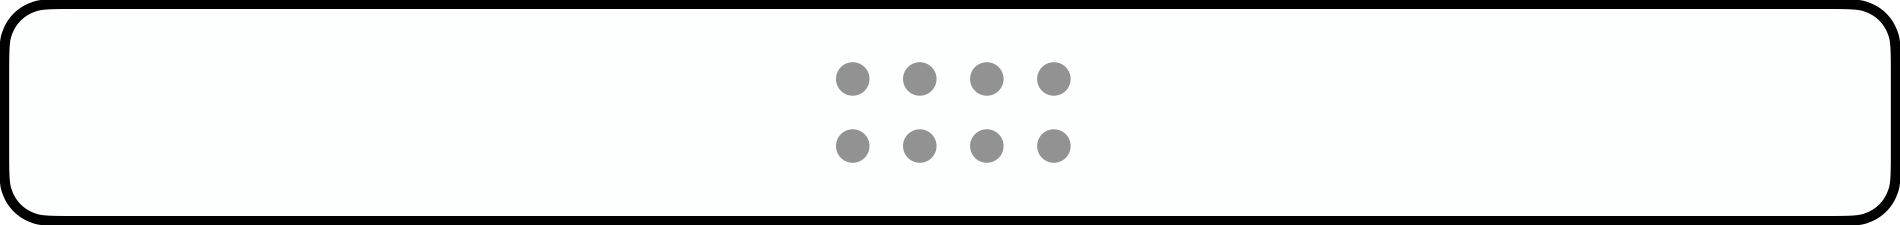
\includegraphics[height=12pt]{Resources/Tenbou/100.png} & \(\times 5\)  \\
	\end{tabular}
	\caption{Recommended point stick distribution.}\label{core:fig:sticks}
\end{figure}

\subsection{Drawing for Seats}\label{core:ssec:seat-draw}

After distribution of point sticks, the seating order of the players must now be determined. There are many ways to do this, three are detailed below. All of these require that you set aside the tiles East, South, West, and North.

\subsubsection*{Direct Draw}\label{core:sssec:direct-draw}

For this draw method, you will only need East, South, West, and North.

\begin{enumerate}
	\item A player will shuffle all four of the tiles face down.
	\item Every other player will draw a tile, leaving the last one to the player who shuffled them.
	\item Each player will take the seat as dictated by their wind, allowing East to choose their seat first. They will be the dealer.
\end{enumerate}

\subsubsection*{Traditional Draw}\label{core:sssec:traditional-draw}

For this draw method, you will need a 1 and a 2 in addition to East, South, West, and North. This method requires everyone to be seated.

\begin{enumerate}
	\item A player will shuffle all six of the tiles face down. Then they will roll both dice.
	\item Counting counter-clockwise, starting from themselves, the player indicated by the dice will be Temporary East.
	\item Temporary East will reveal the tiles and move the numbered tiles outwards to opposite edges.
	\item If the dice roll in step 1 is odd, they will start drawing from the direction of the tile numbered 1. Otherwise they will start drawing from the direction of the tile numbered 2.
	\item Distribute the tiles to each player in the order the tiles are in. Then rearrange the players so that they are seated in the correct order for the winds.
	\item Lastly the Temporary East player will roll the dice one final time to determine the dealer to start the game. 
\end{enumerate}

\subsubsection*{Dealer Only Draw}\label{core:sssec:dealer-only-draw}

For this draw method, you will only need East, South, West, and North. This method works best while everyone is seated already.

\begin{enumerate}
	\item A player will shuffle all four of the tiles face down.
	\item Every other player will draw a tile, leaving the last one to the player who shuffled them.
	\item Whoever draws East will be the dealer, no one needs to move.
\end{enumerate}